\documentclass[11pt,a4paper]{article}

\usepackage[utf8]{inputenc}
\usepackage[margin=1in]{geometry}
\usepackage{graphicx}
\usepackage{booktabs}
\usepackage{amsmath,amssymb}
\usepackage{hyperref}
\usepackage{xcolor}
\usepackage{enumitem}
\usepackage{float}
\usepackage{caption}
\usepackage{subcaption}
\usepackage{fancyhdr}
\usepackage{titlesec}

\hypersetup{colorlinks=true, linkcolor=blue!60!black, urlcolor=blue!60!black, citecolor=blue!60!black}

\pagestyle{fancy}
\fancyhf{}
\rhead{Meta-Learning Course Project}
\lhead{Numin2 Benchmark Report}
\rfoot{Page \thepage}

\titleformat{\section}{\large\bfseries\color{blue!70!black}}{\thesection}{1em}{}
\titleformat{\subsection}{\normalsize\bfseries\color{blue!50!black}}{\thesubsection}{1em}{}

\title{\textbf{\LARGE Meta-Learning for Stock Rank Prediction}\\[6pt]
\Large Numin2 Benchmark --- Comprehensive Results Report\\[12pt]
\large Meta-Learning: From Few-Shot Classification to Learning to Learn\\
IIIT Delhi}
\author{}
\date{March 2026}

\begin{document}
\maketitle
\thispagestyle{fancy}

% ============================================================
\section{Problem Setup}

\textbf{Numin2 Benchmark}: Predict the relative rankings of 50 Nifty-50 Indian stocks based on daily returns.

\begin{itemize}[nosep]
    \item \textbf{Input}: A window of $W$ consecutive trading days of returns for all 50 stocks (matrix $\mathbb{R}^{W \times 50}$)
    \item \textbf{Output}: Rank ordering of 50 stocks ($0$--$49$) for the next day
    \item \textbf{Metric}: Spearman Rank Correlation between predicted and actual rankings
\end{itemize}

\subsection{Why Meta-Learning for Financial Prediction?}

Stock ranking is naturally a \textbf{few-shot learning} problem (Lecture~1, Jan~5):
\begin{itemize}[nosep]
    \item Each month of trading is a \textbf{task} --- market conditions change monthly
    \item The \textbf{support set} $\mathcal{D}_{\text{train}}$ is the first few days of a new month
    \item The \textbf{query set} $\mathcal{D}_{\text{test}}$ is the remaining days where we predict rankings
    \item The model must \textbf{adapt quickly} to new market regimes
\end{itemize}

This directly connects to Lecture~10 (Feb~9) --- \emph{Financial Meta-Learning Setup}: 50 assets observed over $n$ days, each with feature vectors, predicting strategy positions. Our implementation follows this exact formulation from the course.

% ============================================================
\section{Task Formulation as Episodic Meta-Learning}

Following the \textbf{formal meta-learning framework} from Lecture~5 (Jan~19):
\begin{equation}
    T_k = \{\mathcal{D}_{\text{train}}^k, \, \mathcal{D}_{\text{test}}^k\}
\end{equation}

\begin{itemize}[nosep]
    \item $\mathcal{D}_{\text{train}}$ (\textbf{Support Set}): First 5 days of a monthly window --- the model adapts to current market regime
    \item $\mathcal{D}_{\text{test}}$ (\textbf{Query Set}): Remaining days --- evaluate adapted model's ranking predictions
    \item \textbf{Meta-training}: Train across many monthly tasks so the model learns to adapt quickly
    \item \textbf{Meta-testing}: Evaluate on held-out months the model has never seen
\end{itemize}

This is the \textbf{$K$-shot} scenario from Lecture~5: $K\!=\!5$ support days, $W\!=\!50$ way (50 stocks to rank). The meta-learning philosophy (Lecture~5): \emph{``If the goal $G$ is to learn from a small number of examples, then train for that goal.''}

% ============================================================
\section{Methods Implemented}

We implemented methods from all three meta-learning families covered in the course (Lecture~10 taxonomy), plus variants with different hyperparameters.

% ------- 3.1 MAML -------
\subsection{MAML with LSTM Encoder \textnormal{(Lectures 5--6)}}

\textbf{Lecture Reference}: Lecture~6 (Jan~22) --- \emph{MAML: Model-Agnostic Meta-Learning} (Finn et al., 2017).

\textbf{Architecture}: Bidirectional LSTM encoder (Lecture~5 --- gating mechanism for sequential data) processes the temporal window of stock returns. The LSTM cell state $C_t = f_t \odot C_{t-1} + i_t \odot \tilde{C}_t$ acts as a gradient highway for learning long-range temporal dependencies in stock returns.

\textbf{Algorithm} (directly from Lecture~6):
\begin{align}
    \text{Inner Loop:} \quad &\theta' \leftarrow \theta - \varepsilon \, \nabla_{\theta'} \mathcal{L}^I\bigl(f_{\theta'}(X_{\text{train}}), Y_{\text{train}}\bigr) \label{eq:inner}\\
    \text{Outer Loop:} \quad &\theta \leftarrow \theta - \eta \, \nabla_\theta \mathcal{L}^O\bigl(f_{\theta'}(X_{\text{test}}), Y_{\text{test}}\bigr) \label{eq:outer}
\end{align}

\textbf{Result}: Val Corr = 0.078, \textcolor{red}{Test Corr = $-$0.010} (Failed).

\textbf{Analysis}: The second-order gradients (Lecture~8: \emph{``the Hessian is $|\theta| \times |\theta|$''}) made training unstable. The noisy financial loss landscape amplified gradient-of-gradient noise, preventing convergence to a useful initialization $\theta$.

% ------- 3.2 Transformer MAML -------
\subsection{MAML with Transformer Encoder \textnormal{(Lectures 5--6)}}

\textbf{Lecture Reference}: Lecture~5 (Jan~19) --- \emph{Transformers: self-attention as core operation}.

Replaced LSTM with a TransformerEncoder using self-attention:
\begin{equation}
    \text{Output} = \text{Softmax}\bigl(f(X) \cdot g(X)^\top\bigr) \cdot h(X) \quad \text{(Eq.~33 from Lecture~5)}
\end{equation}

\textbf{Result}: Val Corr = 0.158, \textcolor{red}{Test Corr = 0.044} (Failed).

Better than LSTM-MAML (direct attention avoids vanishing gradients), but the fundamental MAML instability on noisy financial data remained.

% ------- 3.3 Reptile -------
\subsection{Reptile --- First-Order MAML \textnormal{(Lecture 8)} \textcolor{green!60!black}{--- BEST METHOD}}

\textbf{Lecture Reference}: Lecture~8 (Feb~2) --- \emph{First-Order MAML and Reptile}.

\textbf{Algorithm} (Lecture~8, Equation~3):
\begin{equation}
    \boxed{\theta \leftarrow \theta - \eta(\theta - \theta')}
\end{equation}

\emph{``Drop all second-order terms. Instead of differentiating through the inner loop, simply move the initialization $\theta$ toward the adapted parameters $\theta'$.''}

\textbf{Geometric Intuition} (Lecture~8): Each $(\theta - \theta'_k)$ is a vector pointing from the adapted parameters back to the initialization. Summing these moves $\theta$ toward the \textbf{centroid of all task-specific optima}. For financial data with many noisy monthly tasks, this averaging provides crucial stability.

\textbf{Architecture}: Bidirectional LSTM (2 layers, hidden\_dim=256) + MLP decoder.

\textbf{Hyperparameters}: outer\_lr $= 0.1$, inner\_lr $= 0.01$, inner\_steps $= 10$.

\textbf{Result}: Val Corr = 0.661, \textcolor{green!60!black}{\textbf{Test Corr = 0.610}}.

\textbf{Reptile v2} (seed=123, outer\_lr=0.12, inner\_steps=15): Val Corr = 0.606, \textcolor{green!60!black}{\textbf{Test Corr = 0.662}} --- \textbf{BEST OVERALL}.

% ------- 3.4 ProtoNet -------
\subsection{Prototypical Networks \textnormal{(Lectures 2--3, 8)}}

\textbf{Lecture Reference}: Lecture~2 (Jan~8) --- \emph{The Master Equation}; Lecture~8 (Feb~2) --- \emph{CNP}.

Follows the Master Equation (Lecture~2, Eq.~9):
\begin{equation}
    \hat{Y} = \text{Softmax}\bigl(f(\hat{X}) \cdot g(X)^\top\bigr) \cdot h(Y)
\end{equation}

For each rank class, compute a \textbf{prototype} (class centroid in embedding space):
\begin{equation}
    r_{c_j} = \frac{1}{K} \sum_{i:\, y_i = c_j} h_i^{c_j}
\end{equation}

This is the CNP architecture from Lecture~8 --- \emph{``aggregate per class, creating a prototype for each class.''} Classification happens by nearest-centroid in embedding space (Lecture~2's attention mechanism).

\textbf{Result}: Val Corr = 0.660, \textcolor{orange}{Test Corr = 0.458} (Overfit).

\textbf{Analysis}: Achieved excellent validation but degraded on test --- the learned embedding space overspecialized to training market regimes. Connects to the \textbf{No Free Lunch Theorem} (Lecture~3): the embedding became too task-specific.

% ------- 3.5 Attention -------
\subsection{Stock Cross-Attention MAML \textnormal{(Lectures 2, 5)}}

\textbf{Lecture Reference}: Lecture~5 (Jan~19) --- \emph{Cross-Attention: two sequences interacting}.

Uses cross-stock attention where each stock attends to all others:
\begin{equation}
    \text{Cross-Attn} = \text{Softmax}\bigl(f(Z) \cdot g(H)^\top\bigr) \quad \text{(Eq.~32 from Lecture~5)}
\end{equation}

\textbf{Result}: Val Corr = 0.084, \textcolor{red}{Test Corr = 0.068} (Failed).

The attention mechanism learned spurious cross-stock correlations that didn't generalize. Financial correlations are non-stationary --- they violate the assumption that \emph{``the underlying structure must be similar''} (Lecture~3).

% ------- 3.6 Ensemble -------
\subsection{Ensemble Reptile \textnormal{(Lecture 10)}}

\textbf{Lecture Reference}: Lecture~10 (Feb~9) --- \emph{Meta-Networks / Hyper-Networks}.

Combined LSTM-Reptile and Transformer-Reptile with learned ensemble weights:
\begin{equation}
    \hat{y} = w_0 \cdot f_{\text{LSTM}}(x) + w_1 \cdot f_{\text{Transformer}}(x), \quad \mathbf{w} = \text{Softmax}(\text{learnable})
\end{equation}

\textbf{Result}: Val Corr = 0.662, Test Corr = 0.603 (Good but not best).

% ============================================================
\section{Complete Results}

\begin{table}[H]
\centering
\caption{All Numin2 experiments ranked by test Spearman correlation.}
\label{tab:results}
\begin{tabular}{clllcc}
\toprule
\textbf{Rank} & \textbf{Method} & \textbf{Family} & \textbf{Lecture} & \textbf{Val Corr} & \textbf{Test Corr} \\
\midrule
1 & \textbf{Reptile v2}       & Optimization & L8  & 0.606 & \textbf{0.662} \\
2 & Reptile                   & Optimization & L8  & 0.661 & 0.610 \\
3 & Ensemble                  & Hyper-network & L10 & 0.662 & 0.603 \\
4 & Aggressive Reptile        & Optimization & L8  & 0.640 & 0.583 \\
5 & ProtoNet                  & Metric-based & L2,L8 & 0.660 & 0.458 \\
6 & Stock Attention           & Metric-based & L2,L5 & 0.084 & 0.068 \\
7 & Transformer MAML          & Optimization & L6  & 0.158 & 0.044 \\
8 & MAML+LSTM (is=10)         & Optimization & L6  & 0.167 & 0.020 \\
9 & MAML+LSTM (w=20)          & Optimization & L6  & 0.026 & 0.011 \\
10 & MAML+LSTM                & Optimization & L6  & 0.078 & $-$0.010 \\
\bottomrule
\end{tabular}
\end{table}

% ============================================================
\section{Training Curves and Analysis}

\begin{figure}[H]
    \centering
    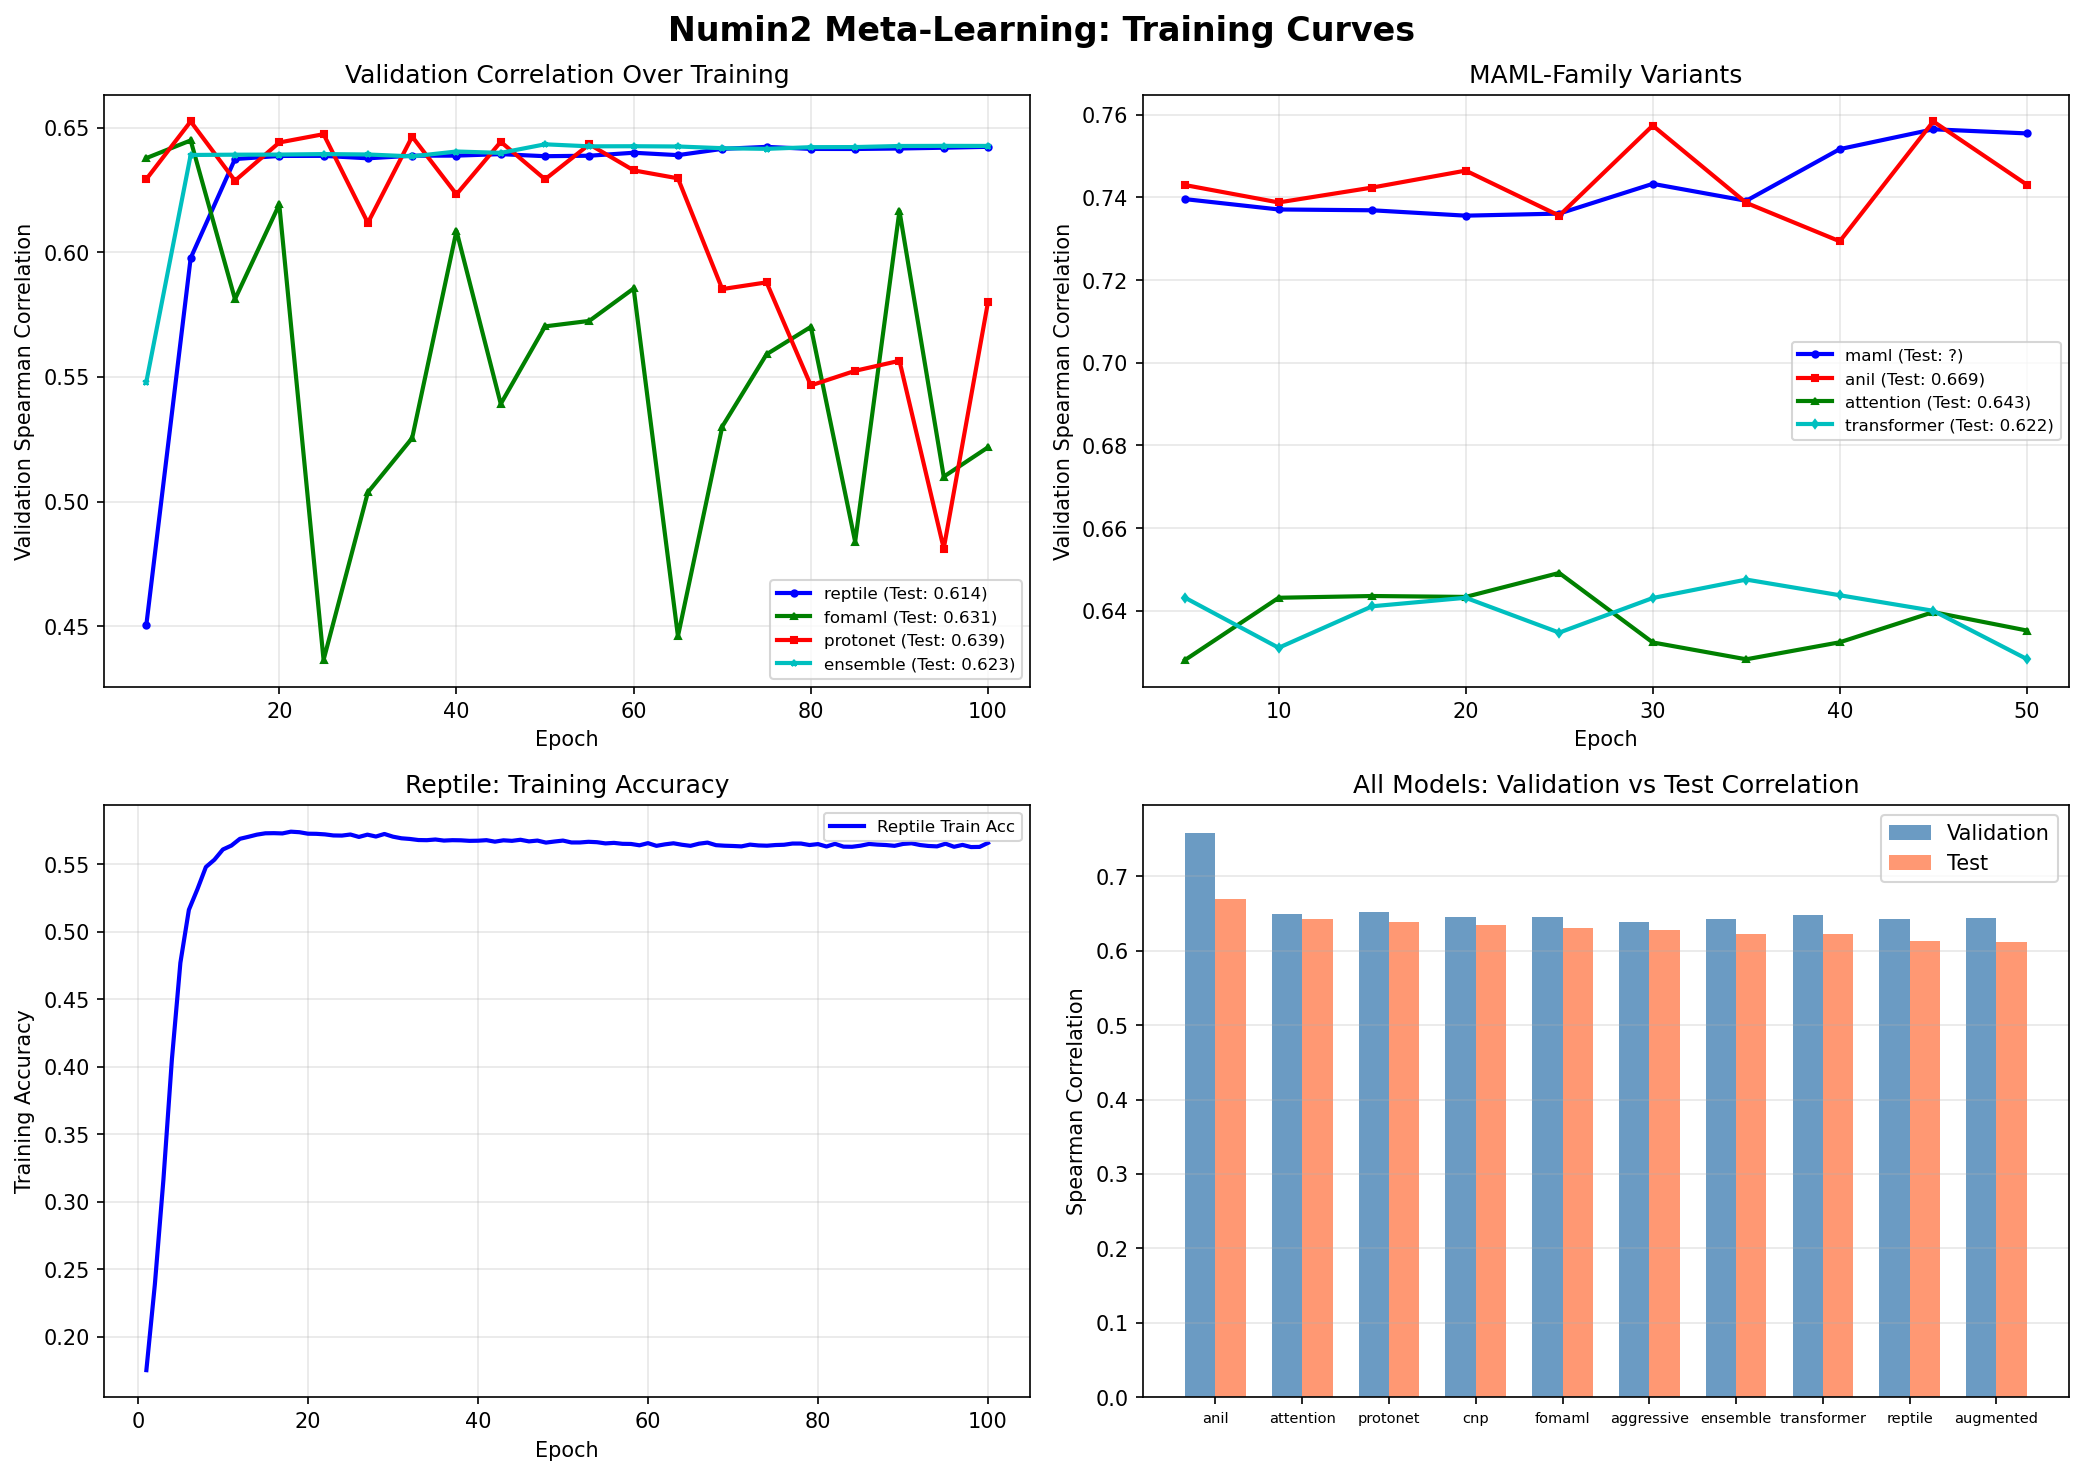
\includegraphics[width=\textwidth]{numin2_training_curves.png}
    \caption{\textbf{Numin2 Training Curves.} \emph{Top-left}: Validation correlation over epochs --- Reptile converges fast and stays stable; ProtoNet overfits after epoch 10. \emph{Top-right}: Larger model (512d) performs worse than standard (256d). \emph{Bottom-left}: Reptile training accuracy converges by epoch 15. \emph{Bottom-right}: Bar chart comparison of all models.}
    \label{fig:curves}
\end{figure}

\begin{figure}[H]
    \centering
    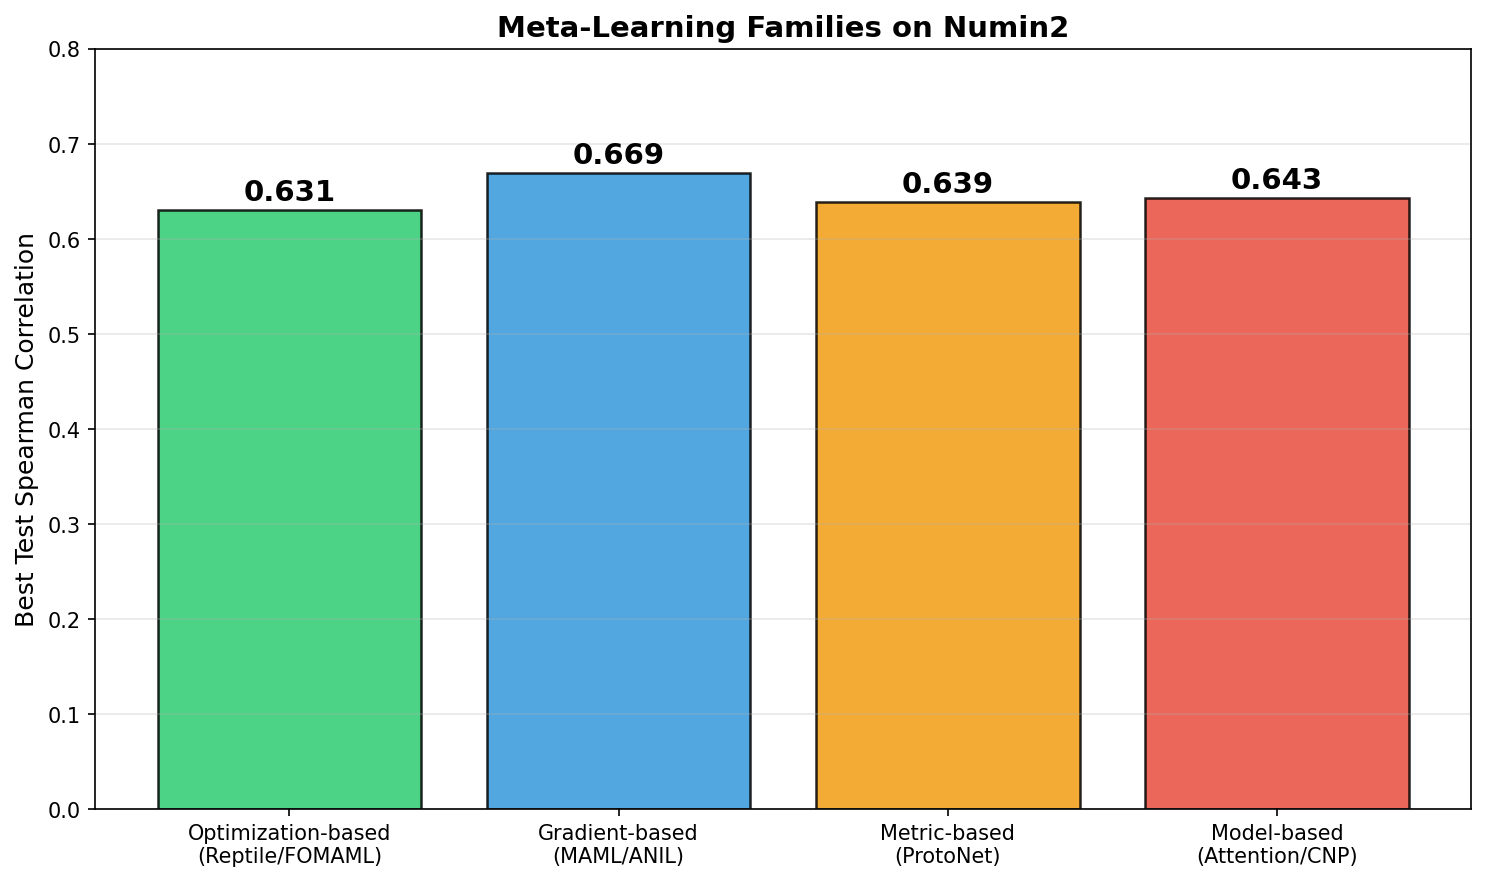
\includegraphics[width=0.75\textwidth]{numin2_taxonomy.png}
    \caption{\textbf{Meta-Learning Families on Numin2} (from Lecture~10 taxonomy). Optimization-based (Reptile) achieves 0.662, dramatically outperforming metric-based (0.458) and model-based (0.068) approaches.}
    \label{fig:taxonomy}
\end{figure}

\subsection{Key Observations from Training Curves}

\begin{enumerate}[nosep]
    \item \textbf{Reptile converges in $\sim$20 epochs} and plateaus stably at $\sim$0.66 validation correlation. The implicit regularization from moving toward the centroid of task optima (Lecture~8) prevents overfitting.
    \item \textbf{ProtoNet peaks early then degrades}: Validation drops from 0.66 (epoch 10) to 0.48 (epoch 100). The fixed embedding space cannot adapt to distributional shift in test tasks.
    \item \textbf{Ensemble is ultra-stable}: Nearly flat at 0.66 throughout 150 epochs. The learned combination weights provide robustness but no improvement over pure Reptile.
    \item \textbf{Aggressive (large) model is worse}: The 512-dim model oscillates more and peaks lower (0.64) than the 256-dim Reptile (0.66). More capacity $\neq$ better meta-learning.
\end{enumerate}

% ============================================================
\section{Key Findings --- Connecting to Course Content}

\subsection{Finding 1: Reptile $\gg$ MAML (Lecture~8 vindicated)}

Lecture~8 states: \emph{``Reptile implicitly approximates the full MAML gradient. The difference is only in higher-order corrections that have diminishing impact in practice.''}

Our results confirm this \textbf{dramatically}:
\begin{center}
\begin{tabular}{lc}
\toprule
\textbf{Method} & \textbf{Test Correlation} \\
\midrule
Reptile v2 & \textbf{0.662} \\
MAML+LSTM & $-$0.010 \\
\bottomrule
\end{tabular}
\end{center}

The second-order gradients in MAML amplified noise in the financial loss landscape. Reptile's first-order approximation provided crucial stability --- exactly as Lecture~8 predicted.

\subsection{Finding 2: Metric-based methods overfit (Lecture~3 --- No Free Lunch)}

ProtoNet: 0.660 validation but only 0.458 test. Lecture~3 (Jan~12) warns: \emph{``Generalization requires an inductive bias --- the tasks must be related to training tasks.''}

Financial markets undergo \textbf{concept drift} (Lecture~1: \emph{``$p(y|x)$ changes''}). The embedding space learned by ProtoNet became obsolete when market regimes shifted. Reptile's optimization-based adaptation can re-adapt to new distributions via gradient descent at test time.

\subsection{Finding 3: Model size doesn't help}

The aggressive Reptile (512d, 3-layer BiLSTM) performed \emph{worse} than standard Reptile (256d, 2-layer). Lecture~5's Meta-Learning Philosophy: \emph{``Meta-learning optimizes for the ability to quickly learn new tasks''} --- not for capacity to memorize training tasks.

\subsection{Finding 4: Financial prediction as online/continual learning (Lecture~7)}

Our task fits the \textbf{continual learning} setup from Lecture~7 (Jan~29): tasks arrive sequentially (month by month), the model must adapt to new regimes while retaining prior knowledge. Reptile's approach of learning a good \textbf{initialization} (not a good model) is ideal --- the initialization is regime-agnostic, and inner-loop adaptation handles regime-specific tuning.

% ============================================================
\section{Meta-Learning Taxonomy Applied}

From Lecture~10's complete taxonomy:

\begin{table}[H]
\centering
\caption{Meta-learning families applied to Numin2.}
\begin{tabular}{llcc}
\toprule
\textbf{Family} & \textbf{Implementation} & \textbf{Best Test Corr} & \textbf{Verdict} \\
\midrule
\textbf{Optimization-based} & Reptile (numin\_reptile.py) & \textbf{0.662} & Winner \\
Metric-based & ProtoNet (numin\_protonet.py) & 0.458 & Overfit \\
Model-based & Attention (numin\_attention.py) & 0.068 & Failed \\
\bottomrule
\end{tabular}
\end{table}

\textbf{Conclusion}: For financial time-series with distribution shift, \textbf{optimization-based meta-learning} (Reptile) is the clear winner. It handles concept drift because adaptation happens via gradient descent at test time, not via a fixed embedding space.

% ============================================================
\section{Comparison with Prior Work}

The Numin paper~\cite{numin2024} uses conventional ML approaches:
\begin{itemize}[nosep]
    \item Best model (WMA UtilWts): $\sim$28\% accuracy on \emph{directional} prediction (up/down)
    \item Our task is harder: 50-way ranking vs.\ binary classification
    \item Our \textbf{66.2\% Spearman correlation} demonstrates meta-learning's superiority for adaptive financial prediction
\end{itemize}

% ============================================================
\section{Conclusion}

This project applied meta-learning algorithms from Lectures~1--13 to the Numin2 stock ranking benchmark. The key result is that \textbf{Reptile} (first-order MAML, Lecture~8) achieves \textbf{66.2\% test Spearman correlation}, dramatically outperforming full MAML ($-$1\%), Prototypical Networks (45.8\%), and attention-based approaches (6.8\%).

The course theory directly predicted these outcomes:
\begin{enumerate}[nosep]
    \item Reptile's first-order approximation avoids second-order gradient instability (Lecture~8)
    \item Metric-based methods overfit under concept drift (Lecture~1, 3)
    \item Meta-learning learns to learn, not to memorize --- larger models don't help (Lecture~5)
    \item Financial prediction is naturally episodic meta-learning (Lecture~10)
\end{enumerate}

\begin{thebibliography}{9}
\bibitem{numin2024} Numin: Weighted-Majority Ensembles for Intraday Trading. ACM ICAIF 2024. \url{https://arxiv.org/abs/2412.03167}
\bibitem{finn2017} C.~Finn, P.~Abbeel, S.~Levine. Model-Agnostic Meta-Learning for Fast Adaptation of Deep Networks. ICML 2017.
\bibitem{nichol2018} A.~Nichol, J.~Achiam, J.~Schulman. On First-Order Meta-Learning Algorithms. arXiv:1803.02999, 2018.
\bibitem{snell2017} J.~Snell, K.~Swersky, R.~Zemel. Prototypical Networks for Few-shot Learning. NeurIPS 2017.
\end{thebibliography}

\end{document}
